%& -shell-escape
%\documentclass[a4paper]{aa}
\documentclass[onecolumn]{aa}
% \documentclass{article}
\usepackage[pagebackref,colorlinks,citecolor=blue,urlcolor=blue,linkcolor=blue]{hyperref}
\usepackage[varg]{txfonts}
\usepackage{graphicx}
\usepackage{natbib}
\usepackage{amssymb}
\usepackage{amsmath}
\usepackage{tikz}
\usetikzlibrary{arrows,positioning,shapes} %,optics}

%\usepackage[squaren,Gray]{SIunits}
\usepackage{siunitx}
%\usepackage{units} % nicefrac
%\newcommand{\units}[1]{$\mathrm{#1}$}

\newcommand{\Oldthorlabs}{SM05PD1B}
\newcommand{\Newthorlabs}{SM05PD3A}

\newcommand{\todo}[1]{\textbf{\textcolor{red}{[#1]}}\xspace}

\usepackage[outputdir={fig},debug]{dot2texi}
\usepackage{draftwatermark}
\usepackage{xspace}
\SetWatermarkText{DRAFT}
\SetWatermarkScale{6}
\SetWatermarkLightness{0.9}
\newcommand{\angexp}{\circ{a}}
\newcommand{\texp}{\ensuremath{\tau}\xspace}
\newcommand{\FixMe}[1]{\textbf{\textcolor{red}{[#1]}}\xspace}
\newcommand{\SZF}[1]{\textbf{\textcolor{blue}{[#1]}}\xspace}
\newcommand{\MARC}[1]{\textbf{\textcolor{green}{[#1]}}\xspace}
\graphicspath{{fig/}}
\makeatletter
\newcommand*\ExpandableInput[1]{\@@input#1 }
\makeatother
\DeclareMathOperator*{\med}{med}
\title{The StarDICE absolute flux calibration experiment: Characterisation of the photometric instrument with a collimated beam projector}

\author{Collaboration Boston Paris}

\abstract{}{}{}{}

\begin{document}

\maketitle

%\section{Currently happening}
%
%\begin{itemize}
%\item SC linearity
%\item pinhole choice
%\item dark current caracterization
%\item Photo-diode change
%\end{itemize}

\tableofcontents

\section{Introduction}


\section{Laboratory setup}

\subsection{StarDice}

\todo{Marc} The StarDICE photometric instrument (SPI) consists in a
Newton telescope with a primary mirror of $40$cm diameter (16'') and
$1.6$m focal length ($f/D = 4$). The focal plane hosts an Andor Ikon-M
954 camera, equipped with a thermoelectrically cooled, deep depleted
and back illuminated CCD sensor (E2V DU934P). The active area of the
sensors is $13.3\times13.3 mm$ divided in $1024\times 1024$ square
pixel of $13\mu m$ side. In this baseline setup, the pixel resolution
is $1.68$ arcsec and the field of view $28.6\times28.6$ arcmin.

The 11cm diagonal is oversized to ensure the fully-illuminated plane
extends over the sensor with a confortable margin in all optical
configurations.

[-0.9240625, -13.120000000000001]

\begin{itemize}
\item Filter-CCD distance: max 40.80 mm, min 26.80 mm
\item field of view $30'x30'$
\item Custom built mount
\item filters $ugrizy$
\end{itemize}

\subsection{CBP}

\todo{Jeremy}

Sketch and/or images the CBP setting

\begin{itemize}
\item Ekspla NT252 tunable laser
\item Light injection system with filters
\item Optical sphere ref
\item Ocean QE65000 spectrograph
\item Photodiode + Keithley 6514. Fig \ref{fig:thorlabs_response}\\
  \emph{Old one} (used in summer 2021 up to 14th of October 2021): Thorlabs
  SM05PD1B with FDS100 spectral response data\\
  \emph{New one} (replaced on the 14th of October 2021): Thorlabs SM05PD3A with
  FD11A spectral response data
  
  \begin{figure}[!ht]
    \begin{center}
      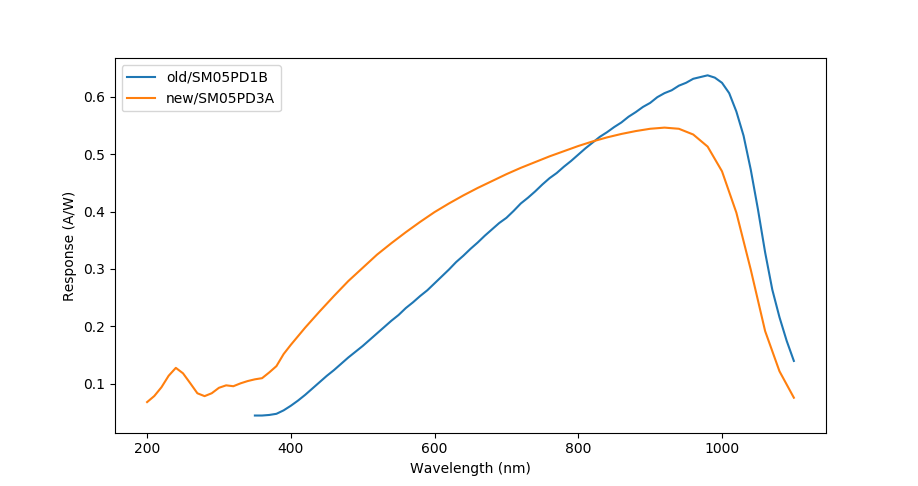
\includegraphics[width=0.8\columnwidth]{thorlabs_response}
    \end{center}
    \caption[]{Response curves of the photodiodes. We see the noticeable
      improvement in the blue for the new one.}
    \label{fig:thorlabs_response}
  \end{figure}
  
  
\item Pinhole slider
\item Telescope: Ritchey Chretien Omegon telescope\\
  Apperture ratio $f/9$\\
  Apperture $154 mm$ \\  
\item Telescope mount
\item Solar Cell on movable mount
\item Keysight B2987A: in order to be able to chop the light at a higher frequency
  than what the Keithley can do. And it is a more contemporary instrument.
\end{itemize}


\subsection{Equations and strategy}

\todo{Thierry}

From equations, draw the data taking plan

with calibrated wavelength

\section{CBP response calibration with a solar cell}

\todo{Jérémy}

Foundations: The Solar Cell QE (Sasha and Elana et al.)


\subsection{Data set description}


\subsubsection{Choice of the dynamic range}
We need to select the number of pulses per wavelength. We decide to keep the
photo-diode current as flat as possible in order to keep the non-linearity of
the Keithley 6514 (that we suppose the largest non-linear component of our
setup) as small as possible.


\begin{figure}[!ht]
\begin{center}
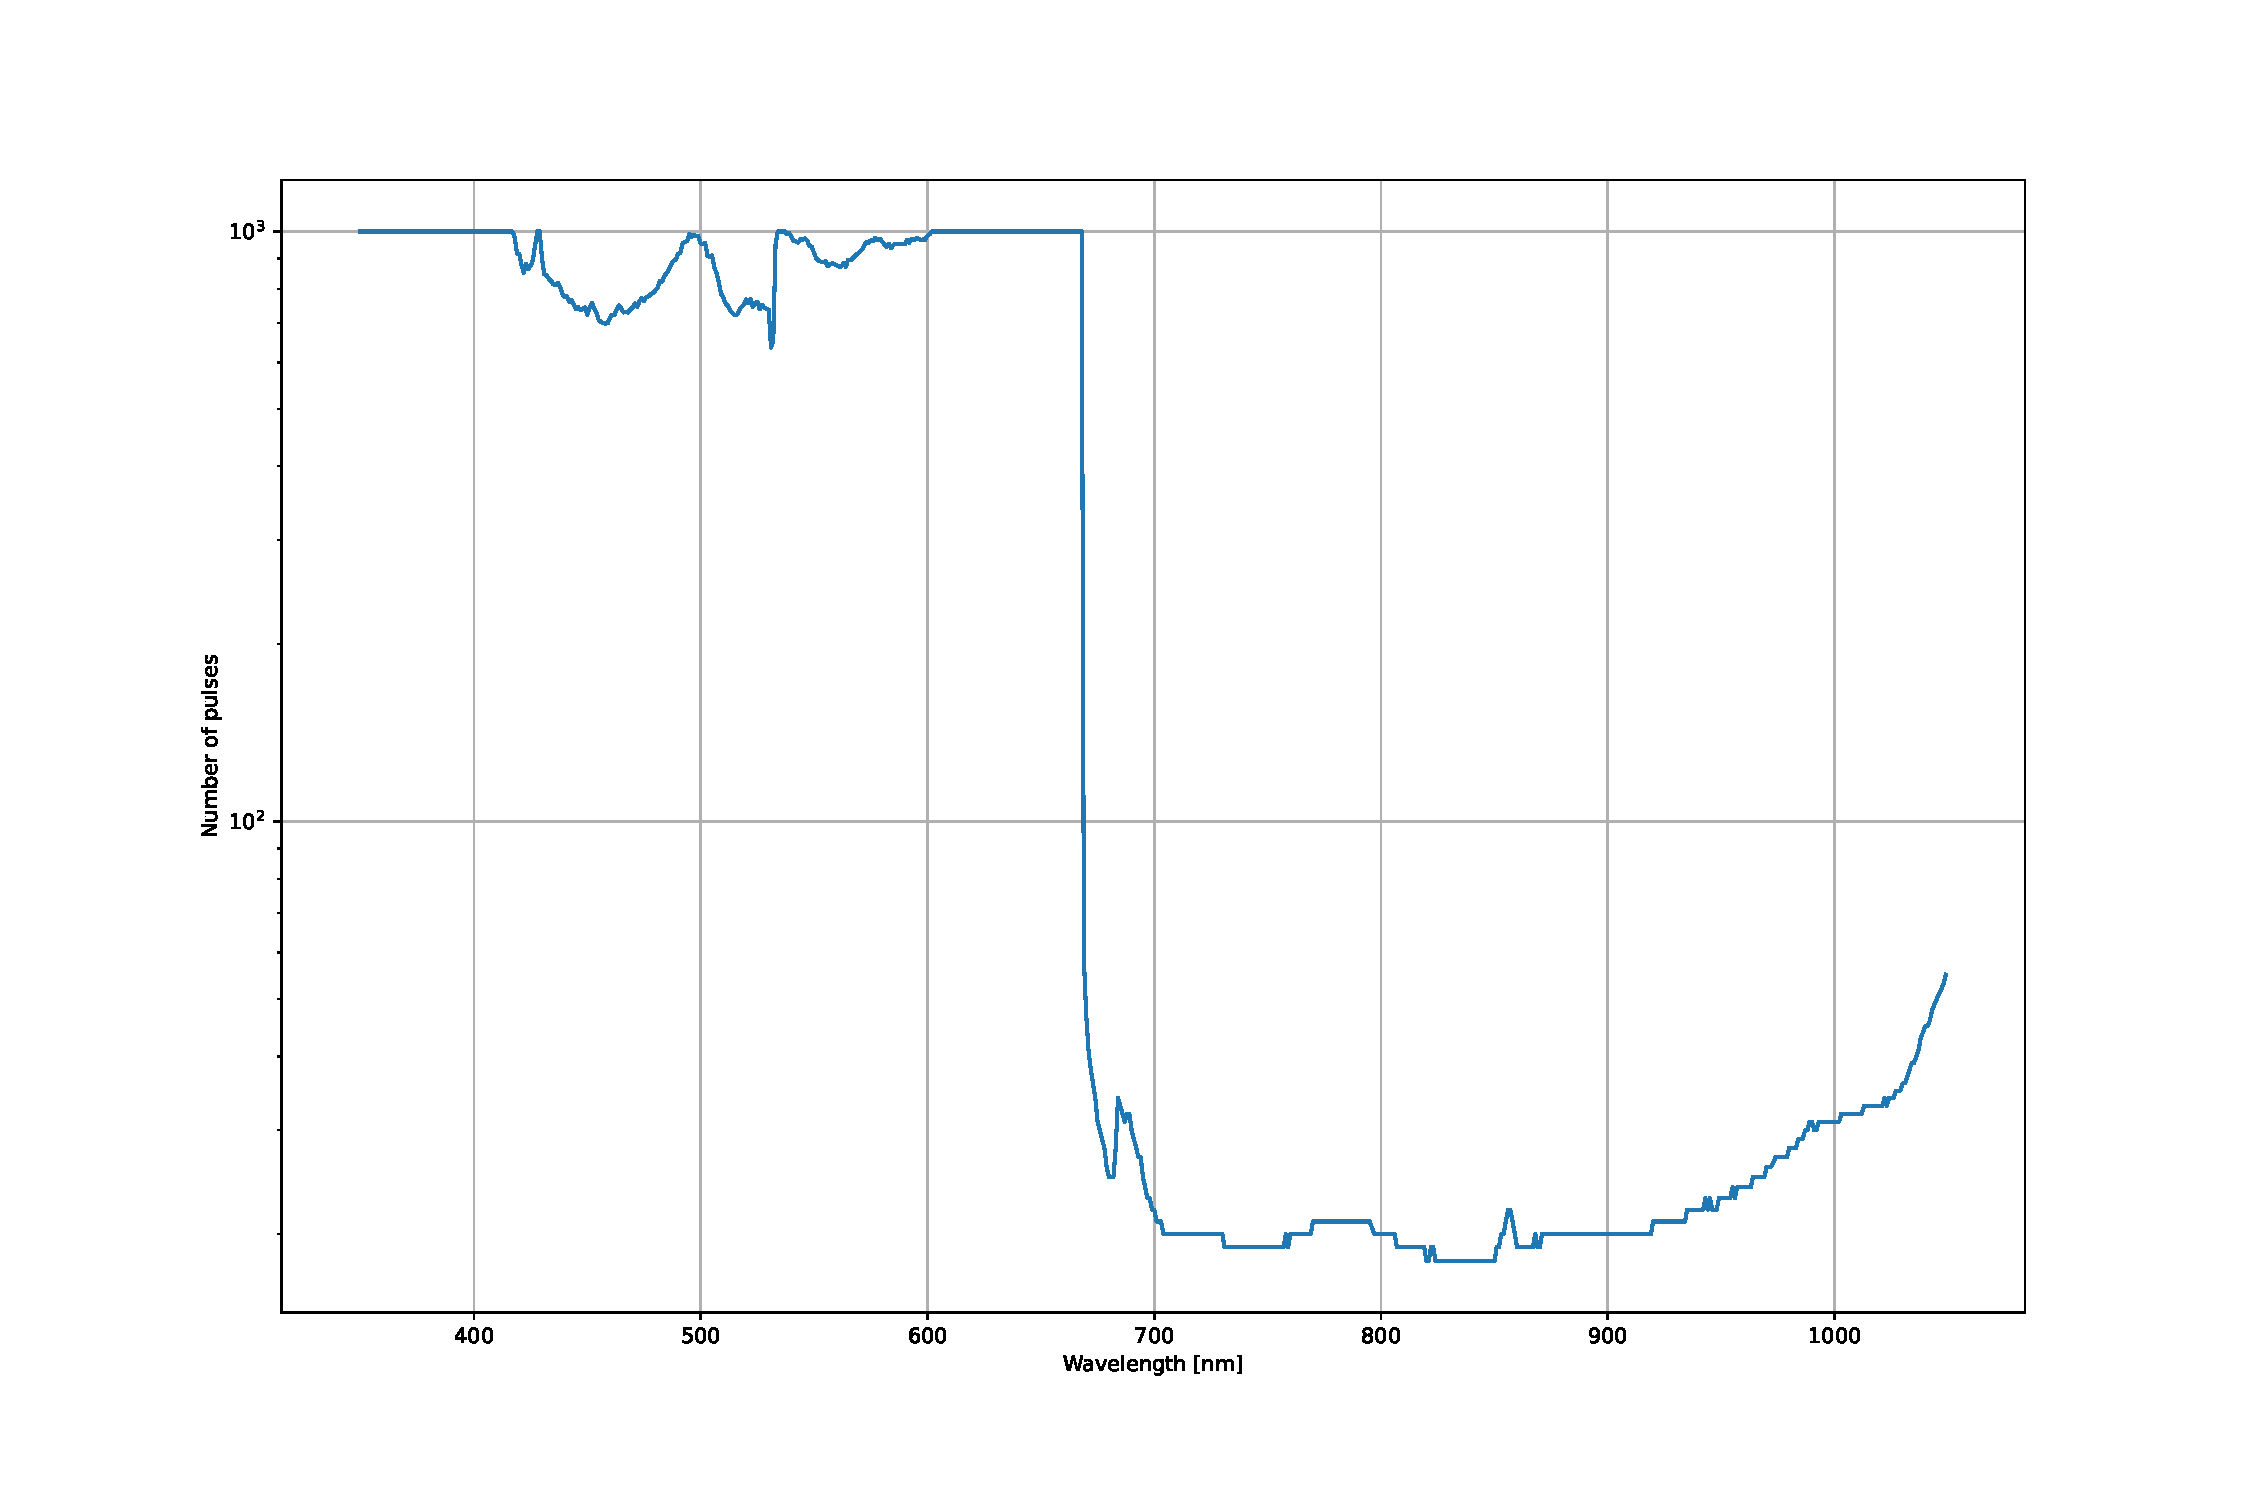
\includegraphics[width=0.8\columnwidth]{calculate_npulses}
\end{center}
\caption[]{Number of pulses per bursts needed to get a constant signal from the photodiode.}
\label{fig:calculate_npulses}
\end{figure}

This was for the Thorlabs \Oldthorlabs


\subsubsection{Dark current characterization}

Measurement and selection of a dark current that doesn't saturate the Keisight
too fast. Measurement of the dark current noise level. 

\begin{itemize}
\item Without offset box: $\sim 20 nA$
\item With offset box: $~ <0> nA \pm 5 nA$
\end{itemize}


Dark current with laser off over 45 minutes, mimicking 10 second observation
blocks corresponding to the 5 laser bursts.
\begin{figure}[!ht]
\begin{center}
%\includegraphics[width=0.8\columnwidth]{dark_current_spectrum.jpeg}
\end{center}
\caption[]{Left: signal auto-correlation. Right: signal FFT. Dominated by the
  stitching of 10 second blocs together.}
\label{fig:darkcurrentspectrum}
\end{figure}

Connecting the Keysight to a $\SI{243}{\ohm}$ resistor gives exactly the same
correlation function. The dark current comes entirely from the Keysight


\subsubsection{Current or charge mode}

\subsubsection{Choice of the pinhole}

\subsubsection{Masking of the beam}
We us a $3/4$ pie-slice mask at the end of the CBP telescope in order to reduce
the beam size, which would otherwile overfill the Solar Cell surface.

Checks to demonstrate that this doesn't impact, via inner reflexions, the
calibration of the CBP telescope.

\subsubsection{Focussing and distance: last focussing 2021-10-11}
The CBP was aligned with the StarDICE telescope to improve the focus. The
StarDICE camera was set close to infinity with no filter (focus encoder:
8mm). The smallest pinhole (75microns). Adjustment of the CBP focus was
performed by Elana in order to get the smallest extension of the pinhole
image. A slight offset was then added to account for the small change in focus
introduce by tightening the locking screws. Here is a confirming image taken
just after.

The focus was check to resist slot changes and even complete removing and
reinstallation of the pinhole.

For the record mount coordinates to get CBP and telescope aligned were
$[13.199987411499023, 1.4999985694885254]$

The measurements at 2 different distances (separated by $16 cm$) show a 5\%
difference in flux both for the 5mm and the 2mm pinhole.

\begin{figure}[!ht]
\begin{center}
%\includegraphics[width=0.8\columnwidth]{distance_variation.png}
\end{center}
\caption[]{The data was taken with the integrating sphere port open. We should
  replace this by more recent data/analysis.}
\label{fig:distancevariation}
\end{figure}


\subsubsection{Available pinholes}

Choice of a pinhole that allows enough S/N. Since we have to switch pinholes,
verification of the relation between flux and pinhole size. Verification of
pinhole achromaticity.

\begin{itemize}
\item Various pinhole sizes measurements with Solar Cell
\item Various pinhole sizes measurement with telescope
\end{itemize}



\subsubsection{Light source filtering}

We suspect that the laser produces harmonics that need to be filtered
out. Measurement of those harmonics and selection of filters to filter them
out. 


\subsubsection{Spectrograph}


\subsection{Data reduction}



\subsubsection{Photodiode data reduction overview}

\subsubsection{Solar Cell data reduction overview}

\subsubsection{Spectro data reduction}


\subsection{CBP response}

\subsection{Systematics}


\subsubsection{External light contamination}

Varying QSW we assume that seen non-linearities come from an external light component

\subsubsection{Varying the SC distance and angle}

to do ???


\subsubsection{Solar Cell linearity}

The Solar Cell has small shunt resistance and we light it with a powerful source
of very short pulse length. Verification of linearity w.r.t flux and w.r.t
number of pulses per burst. 


\begin{itemize}
  \item QSW sequence  (Fig. \ref{fig:SCqswlinearity})
  \item Behavior with change of number of pulses
  \item Behavior of solar cell at different distances
\end{itemize}


\begin{figure}[!ht]
\begin{center}
\includegraphics[width=0.8\columnwidth]{solar_cell_qsw_linearity.jpg}
\end{center}
\caption[]{Something}
\label{fig:SCqswlinearity}
\end{figure}



\section{Instrument model}\label{sec:model}

\todo{Marc: mais plus tard après analyse, et/ou après tuto}

\todo{Direct transmission measurement, ghost brightness model, angle dependence,  Pupil synthesis}

\section{Stardice response}
\label{sec:dataset}

\subsection{Data set description}
\label{sec:datadesc}

\begin{itemize}
\item Images
\item Photocurrent timeseries
\item Spectral time series
\end{itemize}

\subsection{Reduction of images}
\label{sec:photometry}

\todo{phrase pour dire que c'est pareil pour photodiode et spectro}

\subsubsection{5mm pinhole}

\subsubsection{75um pinhole}

\subsubsection{Ghost photometry}

\subsection{Stardice sky response}

\subsubsection{CCD grid}

\subsubsection{Mirror scan}

\subsubsection{Radius scan}

\subsubsection{Ghost buster and beam impact}

\subsubsection{On sky pupil synthesis and filters}



\subsection{Systematic uncertainties}
\label{sec:systematics}

\subsubsection{Stability of the StarDice responses}

\subsubsection{Gain and linearity}
\label{sec:gain}

Varying pinhole with StarDice, and CBP

Varying QSW but depending on result it falls into this subsection or the following

\subsubsection{Pinhole chromaticity}

\subsubsection{Pull distributions}

\subsubsection{Courbes de croissances}


\section{Discussion}

\section{Conclusion}
\label{sec:conclusion}




\end{document}

